\documentclass[tikz]{standalone}
\usepackage{comment}
\usepackage{verbatim}
\usepackage{braket}
\usetikzlibrary{shapes.callouts,arrows,arrows.meta, matrix}
\tikzset{
    level/.style = {
        ultra thick,
        black,
    },
    connect/.style = {
        dashed,
        red
    },
    notice/.style = {
        draw,
        rectangle callout,
        callout relative pointer={#1}
    },
    label/.style = {
        text width=2cm
    },
    detune/.style={draw,dashed,blue},
    arrow/.style={-{latex[scale=1.0]},green,thick},
    fLevel/.style={draw,black}
}

\tikzstyle{doublearr}=[latex-latex, black, line width=0.5pt]
\tikzstyle{arr}=[-latex,black, line width=1pt]

\begin{document}
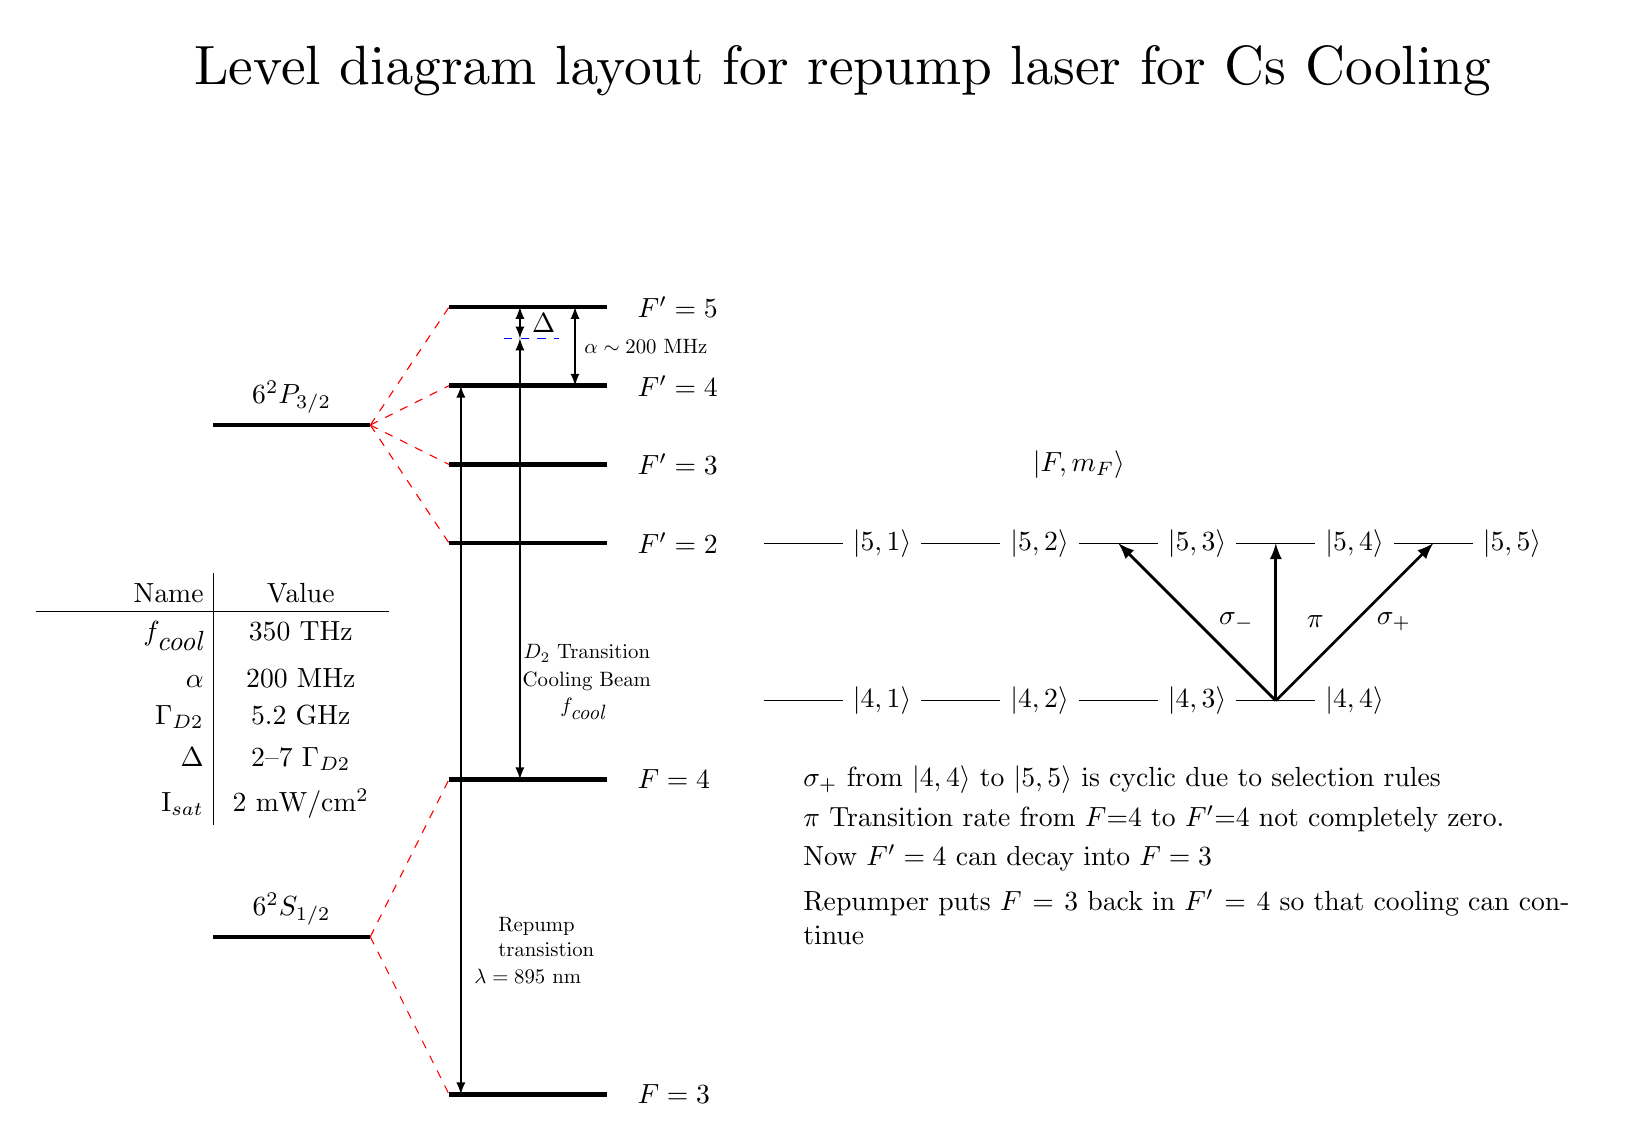
\begin{tikzpicture}
	
	%Draw title
	\node[level, scale = 2] at (8,8){Level diagram layout for repump laser for Cs Cooling};
    
    	
	% Draw 6S level, sublevels and labels
	 \draw[level] (0,-3) -- node[above] {$6^2S_{1/2}$} (2,-3);
   	 \draw[connect] (2,-3) -- (3,-5) (2,-3) -- (3,-1);
   	 \draw[level] (3,-1) --  (5,-1); 
   	 \draw[level] (3,-5) -- (5,-5); 
   	 \node[level,right] at (5.25,-1){$F = 4$};
   	 \node[level,right] at (5.25,-5){$F=3$};
	 %%%%%%%%%%%%%%%%%%%%%%%%%%%%%%%%%%
    
   	% Draw 6P and  F levels with labels
	 \draw[level] (0,3.5) -- node[above] {$6^2P_{3/2}$} (2,3.5);
   	
	 \foreach \i in {2,3,4,5}
	 {
    		\draw[level] (3,\i) -- (5,\i);
		\draw[connect] (2,3.5) -- (3,\i);
		\node[level,right] at (5.25,\i) {$F' = \i$};
	}
	%%%%%%%%%%%%%%%%%%%%%%%%%%%%
	
	% Detuning line and label	
    	\draw[detune] (3.7,4.6)--(4.4,4.6);
    	\node[level] at (4.2,4.8){$\Delta$};
    	\draw[doublearr](3.9,4.6)--(3.9,5);
    
    	% F = 5,4 transisiton
    	\draw[doublearr](4.6,4.0)--(4.6,5);
    	\node[level, scale=0.75] at (5.5,4.5) {$\alpha \sim 200$ MHz};
    	%%%%%%%%%%%%%%%%%%%%%%%%%%%%%%%%%%%%%
    
    	% D2 Transition line and text
    	\draw[doublearr](3.9,-1)--(3.9,4.6);
    	\node[level, scale=0.75] at (4.75,0.6) {$D_2$ Transition};  
     	\node[level, scale=0.75] at (4.75,0.25) {Cooling Beam}; 
    	\node[level, scale=0.75] at (4.7,-0.1){ $f_\textit{cool}$}; 
    	%%%%%%%%%%%%%%%%%%%%%%%%%%%%%%%%%%%%%%
    	
	% Repumping Transition and text
	\draw[doublearr](3.15,-5)--(3.15,4);
	\node[level,scale=0.75, text width=1cm] at (4.0,-3.0) {Repump \\ transistion};
    	\node[level,scale=0.75] at (4.0,-3.5) {$\lambda = 895$ nm};
	%%%%%%%%%%%%%%%%%%%%%%%%%%%%%%%%%%%%%%
	
	% Draw F=4, F=5 level manifold
	\foreach \i in {1,3,5,7,9}
	{
		\draw[fLevel](6 + \i, 2) -- (7+\i,2);
	}
	
	\foreach \i in {1,3,5,7}
	{
		\draw[fLevel](6 + \i, 0) -- (7+\i,0);
	}
	
	\draw[arr](13.5,0)--(15.5,2);
	\draw[arr](13.5,0)--(13.5,2);
	\draw[arr](13.5,0)--(11.5,2);
	
	\node[level] at (11,3){$\ket{F,m_F}$};
	
	\node[level] at (16.5,2){$\ket{5,5}$};
	\node[level] at (14.5,2){$\ket{5,4}$};
	\node[level] at (12.5,2){$\ket{5,3}$};
	\node[level] at (10.5,2){$\ket{5,2}$};
	\node[level] at (8.5,2){$\ket{5,1}$};
	
	\node[level] at (14.5,0){$\ket{4,4}$};
	\node[level] at (12.5,0){$\ket{4,3}$};
	\node[level] at (10.5,0){$\ket{4,2}$};
	\node[level] at (8.5,0){$\ket{4,1}$};

	\node[level] at (15,1){$\sigma_+$};
	\node[level] at (14,1){$\pi$};
	\node[level] at (13,1){$\sigma_-$};
	
	\node[level,scale=1, text width=10cm] at (12.5,-1.0) {$\sigma_+$ from $\ket{4,4}$ to $\ket{5,5}$ is cyclic due to selection rules};
	%\node[level,scale=1, text width=6cm] at (11.0,-1.0) {$\sigma_+$ from $\ket{4,4}$ to $\ket{5,5}$ is cyclic due to selection rules};
	\node[level,scale=1, text width=10cm] at (12.5,-1.5) {$\pi$ Transition rate from $F$=4 to $F'$=4 not completely zero.};
	\node[level,scale=1, text width=10cm] at (12.5,-2.0) {Now $F'=4$ can decay into $F=3$};
	\node[level,scale=1, text width=10cm] at (12.5,-2.75) {Repumper puts $F=3$ back in $F'=4$ so that cooling can continue};
	
	\matrix(dict)[matrix of nodes,%below=of game,
        nodes={align=center,text width=2cm},
        row 1/.style={anchor=south},
        column 1/.style={nodes={text width=2cm,align=right}}
    	]{
        Name & Value\\ %& $b_2$ & $b_3$ & $b_1b_2$ & $b_1b_3$ & $b_2b_3$ & $b_1b_2b_3$\\
        $f_{\textit{cool}}$ & 350 THz \\
        $\alpha$ & $200$ MHz \\
        $\Gamma_{D2}$ &  $5.2$ GHz\\
        $\Delta$ & 2--7 $\Gamma_{D2}$\\
        I$_{sat}$ & 2 mW/cm$^2$\\
    	};
    \draw(dict-1-1.south west)--(dict-1-2.south east);
    \draw(dict-1-1.north east)--(dict-6-1.south east);


%
 %   \draw[connect] (5,3) -- (6,4.5) (5,3) -- (6,3.5) (5,3) -- (6,1.5);
 %   \draw[connect] (5,-2) -- (6,-0.5) (5,-2) -- (6,-1.5) (5,-2) -- (6,-3.5);

  %  \draw[level] (6,4.5) -- node[above] {${}^1P$} (8,4.5);
%%%%%%%%%%%%%%%%%%%%%%%%%%%%%%%%%%%%%%%
\begin{comment}
    \draw[level] (6,3.5) -- node[above] {${}^1D$} (8,3.5);
    \draw[level] (6,1.5) -- node[above] {${}^1F$} (8,1.5);
    \draw[level] (6,-0.5) -- node[above] {${}^3P$} (8,-0.5);
    \draw[level] (6,-1.5) -- node[above] {${}^3D$} (8,-1.5);
    \draw[level] (6,-3.5) -- node[above] {${}^3F$} (8,-3.5);

    \draw[connect] (8,4.5) -- (9,4.5) (8,3.5) -- (9,3.5) (8,1.5) -- (9,1.5);
    \draw[level] (9,4.5) -- (11,4.5) node[right] {${}^1P_1$};
    \draw[level] (9,3.5) -- (11,3.5) node[right] {${}^1D_2$};
    \draw[level] (9,1.5) -- (11,1.5) node[right] {${}^1F_3$};

    \draw[connect] (8,-0.5) -- (9,-0.5) (8,-0.5) -- (9,-0.8) (8,-0.5) -- (9,-1)
        (8,-1.5) -- (9,-1.6) (8,-1.5) -- (9,-1.8) (8,-1.5) -- (9,-1.3)
        (8,-3.5) -- (9,-3.8) (8,-3.5) -- (9,-3.6) (8,-3.5) -- (9,-3.1);
    \foreach \i/\j in {2/-0.5, 1/-0.8, 0/-1} {
        \draw[level] (9,\j) -- (11,\j) node[right] {\scriptsize $\i$};
    }
    \node[level,right] at (11.5,-0.8) {${}^3P_{0,1,2}$};
    \foreach \i/\j in {3/-1.3, 2/-1.6, 1/-1.8} {
        \draw[level] (9,\j) -- (11,\j) node[right] {\scriptsize $\i$};
    }
    \node[level,right] at (11.5,-1.6) {${}^3D_{1,2,3}$};
    \foreach \i/\j in {4/-3.1, 3/-3.6, 2/-3.8} {
        \draw[level] (9,\j) -- (11,\j) node[right] {\scriptsize $\i$};
    }
    \node[level,right] at (11.5,-3.6) {${}^3F_{2,3,4}$};

    % Draw labels
    \node[label] at (4,5.5) {Spin-spin interaction};
    \node[label] at (7,5.5) {Orbit-orbit interaction};
    \node[label] at (10,5.5) {Spin-orbit interaction};

    % Draw annotations
    \node[notice={(0.5,0.5)},text width=1.5cm] at (2,-3) {Hunds rule \# 1};
    \node[notice={(0,1)}] at (4,-4) {Why is triplet lower};
    \node[notice={(0.7,0.7)},text width=3cm] at (6,-5) {Why is higher angular momentum state lower energy?};
    \node[notice={(-0.9,0.9)},text width=1.5cm] at (9,-5) {Hunds rule \# 2};
    \node[notice={(-0.2,1.6)},text width=3cm] at (11,-6.5) {Why is low total angular momentum state lower in energy?};
    \node[notice={(-0.5,0.5)},text width=1.5cm] at (12,-5) {Hunds rule \# 3};
    \end{comment}
    %%%%%%%%%%%%%%%%%%%%%%%%%%%%%%%%%%%%%%%%
\end{tikzpicture}
\end{document}
Output
